\documentclass{TIJMUjiaoanLL}
\pagestyle{empty}


\begin{document}


%课程名称
\kecheng{系统生物学}
%课程内容
\neirong{转录组学(顺反组与表观遗传学)\ /\ 第3章}
%教师姓名
\jiaoshi{伊现富}
%职称
\zhicheng{讲师}
%教学日期(格式:XXXX年XX月XX日XX时-XX时)
\riqi{2017年3月13日10:00-12:00}
%授课对象(格式:XXX系XXXX年级XX班(硕/本/专科))
\duixiang{生物医学工程与技术学院2014级生信班(本)}
%听课人数
\renshu{30}
%授课方式
\fangshi{理论讲授}
%学时数
\xueshi{2}
%教材版本
\jiaocai{系统生物学,第1版}


%教案首页
\firstHeader
\maketitle
\thispagestyle{empty}

\mudi{
\begin{itemize}
  \item 掌握ChIP-Seq的分析流程,Methyl-Seq的分析流程。
  \item 熟悉顺反组的基本概念,表观遗传学的基本概念。
  \item 了解ChIP-Seq的实验流程,Methyl-Seq的实验流程。
  \item 自学研究顺反组的其他方法,研究表观遗传学的其他方法。
\end{itemize}
}

\fenpei{
\begin{itemize}
  \item (5')引言与导入:回顾二代测序技术及其应用。
  \item (45')顺发组:介绍顺反组的概念,讲解ChIP-Seq的实验方法与分析流程,解释Peak calling的基本原理,总结ChIP-Seq的主要应用和数据分析的常用工具,介绍ChIP-Seq的应用实例。
  \item (45')表观遗传学:介绍表观遗传学的概念和主要内容,介绍DNA甲基化,讲解Methyl-Seq的实验方法与分析流程,总结Methyl-Seq数据分析的常用工具,介绍Methyl-Seq的应用实例。
  \item (5')总结与答疑:总结授课内容中的知识点与技能,解答学生疑问。
\end{itemize}
}

\zhongdian{
\begin{itemize}
  \item 重点:ChIP-Seq数据分析的基本流程,Methyl-Seq数据分析的基本流程。
  \item 难点:Peak Calling的基本原理。
  \item 解决策略:通过实例讲解和比较类比帮助学生理解、记忆。
\end{itemize}
}

\waiyu{
  \vspace*{-10pt}
  \begin{multicols}{2}
    顺反组(cistrome)

    染色质免疫沉淀-测序(ChIP-Seq)

    表观遗传学(epigenetics)

    DNA甲基化(DNA methylation)

    亚硫酸盐测序(bisulfite sequencing)
  \end{multicols}
  \vspace*{-10pt}
}

\fuzhu{
\begin{itemize}
  \item 多媒体:ChIP-Seq的实验方法和分析工具,Peak calling的基本原理,Methyl-Seq的实验方法和分析工具。
  \item 板书:ChIP-Seq的分析流程,Methyl-Seq的分析流程。
\end{itemize}
}

\sikao{
  \vspace*{-10pt}
  \begin{multicols}{2}
  \begin{itemize}
    \item 什么是顺反组?
    \item 解释Peak calling的基本原理。
    \item 总结ChIP-Seq的分析流程和常用工具。
    \item 什么是表观遗传学?
    \item 什么是DNA甲基化?
    \item 总结Methyl-Seq的分析流程和常用工具。
  \end{itemize}
  \end{multicols}
  \vspace*{-10pt}
}

\cankao{
\begin{itemize}
  \item 维基百科等网络资源。
\end{itemize}
}

\firstTail


%教案续页
\newpage
\otherHeader

\begin{enumerate}
  \item 引言与导入(5分钟)
    \begin{itemize}
\parpic[fr]{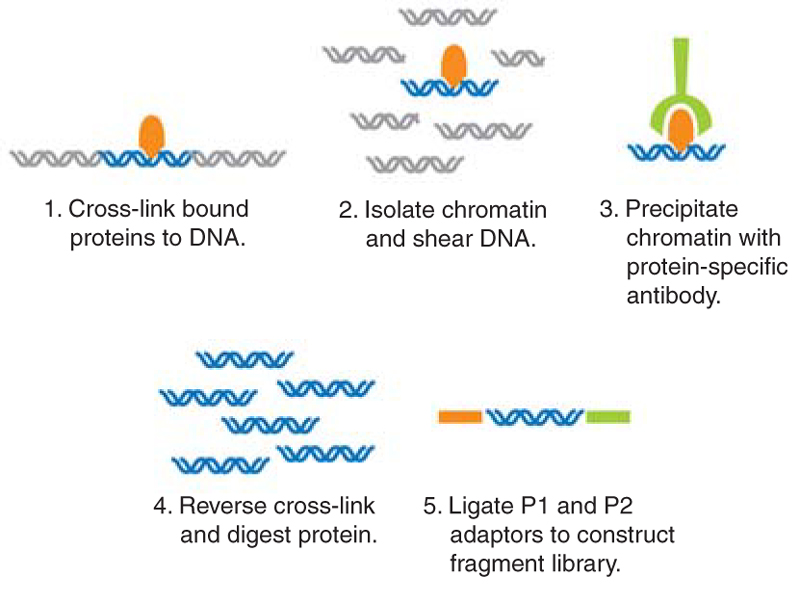
\includegraphics[width=5cm]{c3.chipseq.exp.02.jpg}}
      \item 二代测序技术:Roche/454,Illumina/Solexa,ABI/SOLiD
      \item 二代测序应用:外显子组测序,全基因组测序,RNA-Seq
    \end{itemize}

  \item 顺反组(45分钟)
    \begin{enumerate}
      \item 顺反组简介
        \begin{itemize}
          \item 基本概念:全基因组尺度下反式作用因子的顺式作用靶点的集合
          \item 研究方法:ChIP-on-chip,ChIP-Seq
        \end{itemize}
      \item ChIP-Seq\textcolor{red}{(与RNA-Seq进行对比)}
        \begin{enumerate}
\parpic[fr]{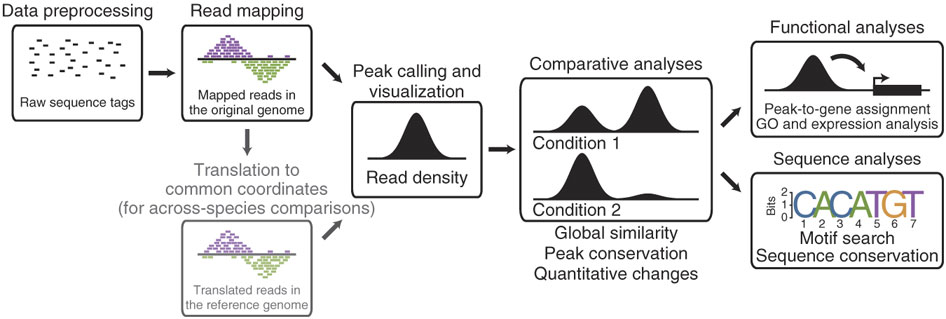
\includegraphics[width=9cm]{c3.chipseq.bx.04.jpg}}
          \item 基本概念:分析蛋白质与DNA的交互作用
          \item 实验流程:ChIP $\Rightarrow$ Sequencing
          \item \textcolor{red}{【重点】}分析流程:QC $\Rightarrow$ Mapping $\Rightarrow$ Peak calling $\Rightarrow$ Annotation
          \item \textcolor{red}{【难点】}Peak calling
            \begin{itemize}
\parpic[fr]{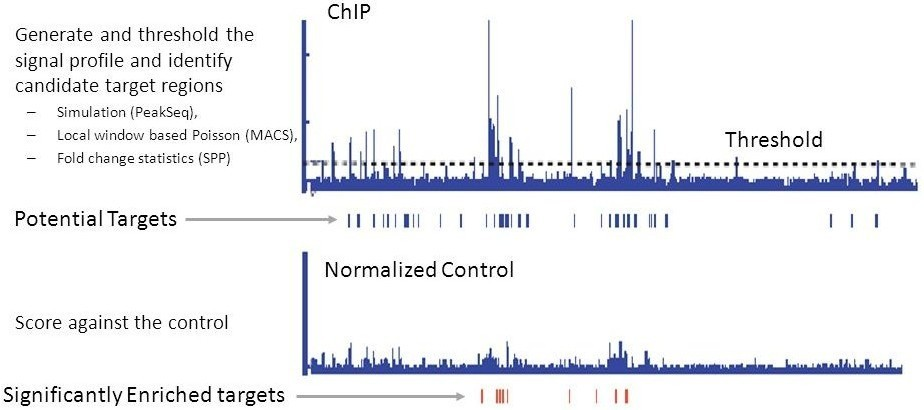
\includegraphics[width=9cm]{c3.chipseq.pc.02.jpg}}
              \item 基本概念:用于鉴定经染色质免疫沉淀-测序或 MeDIP-测序实验后所得到的比对读段富集在基因组哪些区域中的一种计算方法
              \item Differential peak calling: one stage vs. two stage
            \end{itemize}
          \item 常用工具:MACS,PeakSeq,HOMER,MEME\textcolor{red}{(流程 vs. 工具 vs. 实例)}
% \parpic[fr]{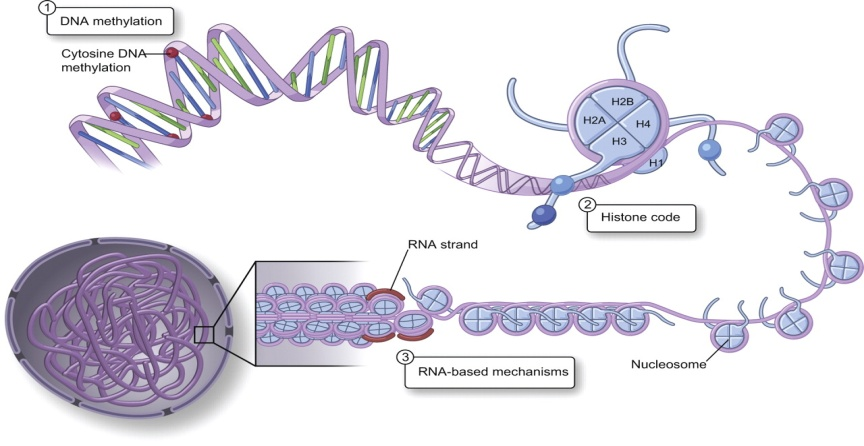
\includegraphics[width=9cm]{c3.epi.intro.02.jpg}}
          \item 应用实例:Nucleosome,TF
        \end{enumerate}
    \end{enumerate}

  \item 表观遗传学(45分钟)
    \begin{enumerate}
      \item 表观遗传学简介
        \begin{enumerate}
          \item 表观遗传学
            \begin{itemize}
\parpic[fr]{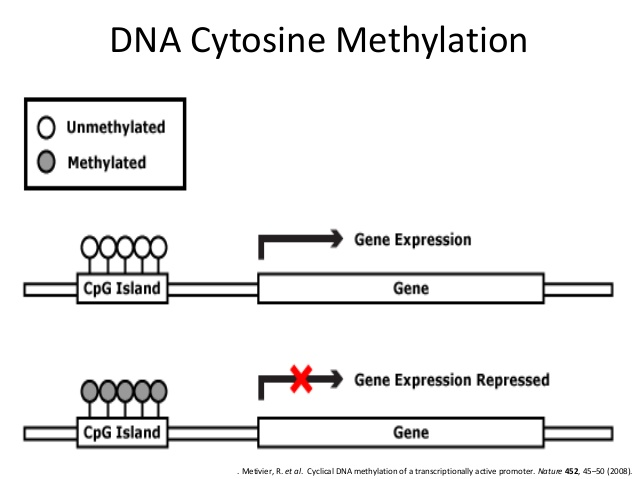
\includegraphics[width=6.5cm]{c3.epi.methy.01.jpg}}
              \item 基本概念:在不改变DNA序列的前提下,通过某些机制引起可遗传的基因表达或细胞表现型的变化
              \item 主要机制:DNA甲基化、组蛋白修饰、RNA干扰等
            \end{itemize}
          \item DNA甲基化
            \begin{itemize}
              \item 基本概念:DNA化学修饰的一种形式
              \item 研究方法:亚硫酸盐测序
            \end{itemize}
        \end{enumerate}
      \item Methyl-Seq\textcolor{red}{(与ChIP-Seq进行类比)}
        \begin{enumerate}
\parpic[fr]{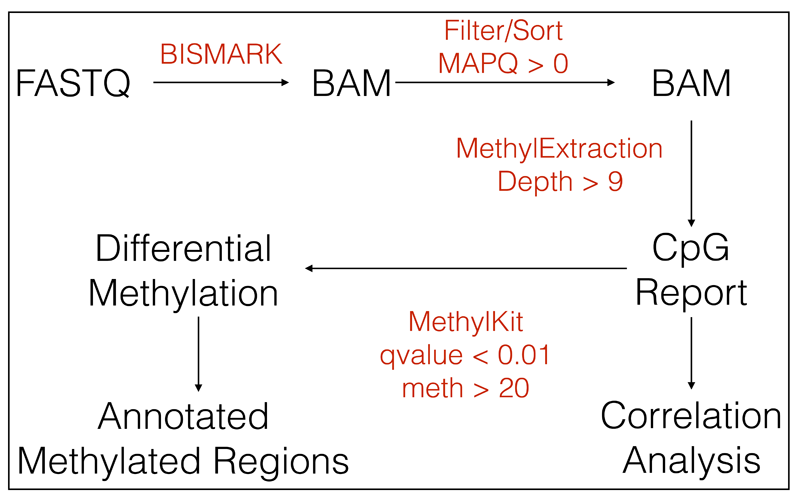
\includegraphics[width=6.5cm]{c3.mseq.bx.02.png}}
          \item 实验流程:DNA fragment $\Rightarrow$ bisulfite conversion $\Rightarrow$ Sequencing
          \item \textcolor{red}{【重点】}分析流程:QC $\Rightarrow$ Mapping $\Rightarrow$ Differential Methylation $\Rightarrow$ Annotation
          \item 常用工具:Bismark,bwa-meth,methylKit
          \item 应用实例\textcolor{red}{(讲解实例的同时回顾/总结分析流程,介绍常用工具)}
        \end{enumerate}
    \end{enumerate}

\otherTail
\newpage
\otherHeader

  \item 总结与答疑(5分钟)
    \begin{enumerate}
      \item 知识点
	\begin{itemize}
    \item 顺反组:基本概念,ChIP-Seq流程,常用工具,Peak calling原理
    \item 表观遗传学:基本概念,Methyl-Seq流程,常用工具
	\end{itemize}
      \item 技能
	\begin{itemize}
    \item 对ChIP-Seq数据进行分析
    \item 对Methyl-Seq数据进行分析
	\end{itemize}
    \end{enumerate}
\end{enumerate}

\otherTail


\end{document}

